\documentclass{ntuabeamer}
\usepackage[utf8]{inputenc}
\usepackage{amsmath,amssymb,tikz}
\usetikzlibrary{arrows.meta,positioning}

\title{Physics-Informed Neural Networks and Neural Operators}
\author{}
\date{}

\definecolor{courseblue}{HTML}{3F7CAC}
\definecolor{courseorange}{HTML}{D97706}
\definecolor{coursegreen}{HTML}{27864A}
\definecolor{coursegray}{HTML}{667085}
\definecolor{coursepurple}{HTML}{7656A3}
\definecolor{coursered}{HTML}{B5473C}
\definecolor{courselightblue}{HTML}{DCE9F5}
\definecolor{courselightorange}{HTML}{F9E4C8}
\tikzset{
  flow/.style={-{Latex[length=3mm]},very thick,courseblue},
  box/.style={draw,rounded corners,very thick,align=center,minimum width=1.8cm,minimum height=0.9cm}
}

\begin{document}
\begin{frame}[plain]\makepresentationtitle\end{frame}

\begin{frame}{A PDE Problem Includes More Than an Equation}
  Find a field \(u:\Omega\to\mathbb R\) such that
  \[
    \mathcal N[u](\mathbf x)=f(\mathbf x),
    \qquad \mathbf x\in\Omega,
  \]
  with boundary and initial conditions
  \[
    \mathcal B[u](\mathbf x)=g(\mathbf x),
    \quad \mathbf x\in\partial\Omega,
    \qquad
    u(\mathbf x,0)=u_0(\mathbf x).
  \]
  \begin{itemize}
    \item \(\mathcal N\) may contain spatial and temporal derivatives.
    \item Coefficients, geometry, forcing, and conditions define the instance.
    \item A small residual does not by itself imply a useful solution.
  \end{itemize}
\end{frame}

\begin{frame}{A PINN Represents One Solution Field}
  \[
    u_\theta(\mathbf x,t)\approx u(\mathbf x,t).
  \]
  \centering
  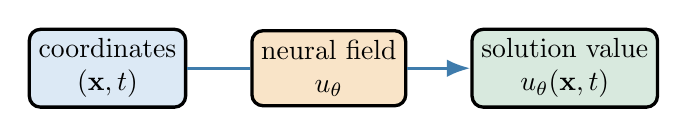
\begin{tikzpicture}[node distance=0.8cm]
    \node[box,fill=courselightblue] (x) {coordinates\\\((\mathbf x,t)\)};
    \node[box,fill=courselightorange,right=of x] (net) {neural field\\\(u_\theta\)};
    \node[box,fill=coursegreen!18,right=of net] (u) {solution value\\\(u_\theta(\mathbf x,t)\)};
    \draw[flow] (x)--(net)--(u);
  \end{tikzpicture}
  \vspace{0.6cm}
  \begin{itemize}
    \item Inputs are coordinates, not a fixed mesh index.
    \item Parameters \(\theta\) are optimized for this PDE instance.
    \item The differential equation supplies training constraints.
  \end{itemize}
\end{frame}

\begin{frame}{Automatic Differentiation Produces PDE Derivatives}
  If \(u_\theta(x,t)\) is differentiable,
  \[
    \partial_t u_\theta,\qquad
    \nabla u_\theta,\qquad
    \nabla^2u_\theta
  \]
  follow by repeated chain rule through the network.
  \[
    u_\theta(x)=W_2\phi(W_1x+b_1)+b_2
    \quad\Longrightarrow\quad
    \frac{du_\theta}{dx}
      =W_2\operatorname{diag}(\phi')W_1.
  \]
  \begin{itemize}
    \item Derivatives are exact for the represented computation up to floating-point error.
    \item They are not exact derivatives of the unknown physical solution.
    \item Smooth activations are needed when the residual uses higher derivatives.
  \end{itemize}
\end{frame}

\begin{frame}{Collocation Converts the PDE Into Residual Samples}
  Define the interior residual
  \[
    r_\theta(\mathbf x,t)
      =\mathcal N[u_\theta](\mathbf x,t)-f(\mathbf x,t).
  \]
  At collocation points \(\{(\mathbf x_i,t_i)\}_{i=1}^{N_r}\),
  \[
    L_{\mathrm{PDE}}(\theta)
      =\frac1{N_r}\sum_{i=1}^{N_r}
       |r_\theta(\mathbf x_i,t_i)|^2.
  \]
  \begin{itemize}
    \item Collocation points need no observed solution values.
    \item Sampling determines where the equation is enforced.
    \item Zero sampled residual does not guarantee zero residual between points.
  \end{itemize}
\end{frame}

\begin{frame}{The Objective Combines Distinct Constraints}
  \[
    \boxed{
    L=\lambda_rL_{\mathrm{PDE}}
      +\lambda_bL_{\mathrm{BC}}
      +\lambda_0L_{\mathrm{IC}}
      +\lambda_dL_{\mathrm{data}} }.
  \]
  \[
    L_{\mathrm{BC}}
      =\frac1{N_b}\sum_i
        |\mathcal B[u_\theta](\mathbf x_i)-g(\mathbf x_i)|^2,
    \qquad
    L_{\mathrm{data}}
      =\frac1{N_d}\sum_i|u_\theta(\mathbf x_i)-y_i|^2.
  \]
  \begin{itemize}
    \item The terms have different units, scales, and gradient magnitudes.
    \item Weights change the optimization problem, not only presentation.
  \end{itemize}
\end{frame}

\begin{frame}{Nondimensionalization Makes Scales Comparable}
  Choose characteristic scales \(x=L\widehat x\), \(t=T\widehat t\), \(u=U\widehat u\).
  For
  \[
    \partial_tu-\nu\,\partial_{xx}u=0,
  \]
  substitution gives
  \[
    \partial_{\widehat t}\widehat u
      -\underbrace{\frac{\nu T}{L^2}}_{\text{dimensionless group}}
       \partial_{\widehat x\widehat x}\widehat u=0.
  \]
  \begin{itemize}
    \item Coordinate scales affect derivatives and gradients.
    \item Dimensionless variables expose the relevant physical ratios.
    \item Loss weights still require monitoring after nondimensionalization.
  \end{itemize}
\end{frame}

\begin{frame}{Worked Example: A One-Dimensional Boundary Problem}
  \[
    -u''(x)=\pi^2\sin(\pi x),
    \qquad x\in(0,1),
  \]
  \[
    u(0)=u(1)=0.
  \]
  The exact solution is
  \[
    \boxed{u(x)=\sin(\pi x)}
  \]
  because
  \[
    -\frac{d^2}{dx^2}\sin(\pi x)=\pi^2\sin(\pi x).
  \]
  \begin{itemize}
    \item This example separates residual enforcement from boundary enforcement.
  \end{itemize}
\end{frame}

\begin{frame}{Soft Constraints Penalize Boundary Error}
  For the boundary-value example,
  \[
    r_\theta(x)=-u_\theta''(x)-\pi^2\sin(\pi x),
  \]
  \[
    L(\theta)
      =\frac1{N_r}\sum_i r_\theta(x_i)^2
       +\lambda_b\big(u_\theta(0)^2+u_\theta(1)^2\big).
  \]
  \begin{itemize}
    \item Any network output is admissible during optimization.
    \item Finite \(\lambda_b\) permits boundary error.
    \item Very large \(\lambda_b\) can make the optimization poorly balanced.
  \end{itemize}
\end{frame}

\begin{frame}{Hard Constraints Satisfy Boundaries by Construction}
  Use the trial solution
  \[
    \boxed{u_\theta(x)=x(1-x)N_\theta(x)}.
  \]
  Then
  \[
    u_\theta(0)=u_\theta(1)=0
  \]
  for every \(\theta\).
  \begin{itemize}
    \item Only the interior residual needs optimization.
    \item The construction must match the exact boundary form.
    \item Complex geometry or mixed conditions can make hard constraints difficult.
  \end{itemize}
\end{frame}

\begin{frame}{Inverse Problems Treat Physical Parameters as Unknowns}
  Suppose
  \[
    -\kappa u''(x)=f(x)
  \]
  and sparse measurements of \(u\) are available. Optimize
  \[
    L(\theta,\kappa)
      =L_{\mathrm{PDE}}(\theta,\kappa)
       +\lambda_dL_{\mathrm{data}}(\theta).
  \]
  Enforce positivity structurally:
  \[
    \kappa=\operatorname{softplus}(\rho)>0.
  \]
  \begin{itemize}
    \item Jointly fitting \(u_\theta\) and \(\kappa\) does not ensure identifiability.
    \item Measurements and excitation must contain information about \(\kappa\).
  \end{itemize}
\end{frame}

\begin{frame}{PINNs Can Fail Even When the Formulation Is Correct}
  \begin{itemize}
    \item Stiff equations create widely separated derivative scales.
    \item Spectral bias makes high-frequency components difficult to fit.
    \item Composite loss terms can produce conflicting gradients.
    \item Sparse collocation can miss localized residuals or shocks.
    \item Nonconvex optimization may settle at a poor residual balance.
    \item Discontinuous solutions conflict with smooth network assumptions.
  \end{itemize}
  \[
    \text{physical constraint}\neq\text{automatic numerical reliability}.
  \]
\end{frame}

\begin{frame}{Validation Must Be Independent of the Training Residual}
  Evaluate on new points and physical quantities:
  \[
    E_u=\left(
      \frac{\sum_j|u_\theta(\mathbf x_j)-u_{\mathrm{ref}}(\mathbf x_j)|^2}
           {\sum_j|u_{\mathrm{ref}}(\mathbf x_j)|^2}
    \right)^{1/2},
  \]
  \[
    E_r=\left(\frac1{N_{\mathrm{val}}}
      \sum_j|r_\theta(\mathbf x_j)|^2\right)^{1/2}.
  \]
  \begin{itemize}
    \item Use collocation points not seen during training.
    \item Check boundary error, conservation, and convergence under denser sampling.
    \item Compare with an established numerical reference when available.
  \end{itemize}
\end{frame}

\begin{frame}{A Neural Operator Learns a Family of Solution Maps}
  A PDE solution operator maps an input function to an output function:
  \[
    \boxed{\mathcal G:a(\cdot)\mapsto u(\cdot)}.
  \]
  Examples of \(a\):
  \begin{itemize}
    \item forcing \(f(\mathbf x)\),
    \item coefficient field \(a(\mathbf x)\),
    \item initial condition \(u_0(\mathbf x)\),
    \item boundary data or geometry description.
  \end{itemize}
  \[
    \mathcal G_\theta(a)\approx\mathcal G(a)
    \quad\text{over a distribution of inputs}.
  \]
\end{frame}

\begin{frame}{Operator Learning Amortizes Repeated Solves}
  \centering
  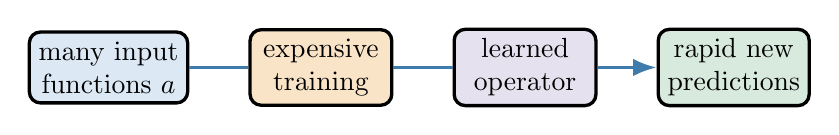
\begin{tikzpicture}[node distance=0.75cm]
    \node[box,fill=courselightblue] (inputs) {many input\\functions \(a\)};
    \node[box,fill=courselightorange,right=of inputs] (train) {expensive\\training};
    \node[box,fill=coursepurple!18,right=of train] (operator) {learned\\operator};
    \node[box,fill=coursegreen!18,right=of operator] (outputs) {rapid new\\predictions};
    \draw[flow] (inputs)--(train)--(operator)--(outputs);
  \end{tikzpicture}
  \vspace{0.7cm}
  \begin{itemize}
    \item Training requires many solved instances or physics-based constraints.
    \item Inference can be fast for new inputs from the trained distribution.
    \item Amortization helps only when repeated related solves are needed.
  \end{itemize}
\end{frame}

\begin{frame}{Resolution Independence Requires More Than New Grid Size}
  A continuous operator acts between function spaces:
  \[
    \mathcal G:\mathcal A\to\mathcal U.
  \]
  Its implementation observes finite samples
  \[
    \{a(\mathbf x_i)\}_{i=1}^{N}
    \quad\longmapsto\quad
    \{\widehat u(\mathbf y_j)\}_{j=1}^{M}.
  \]
  \begin{itemize}
    \item Training on arrays alone does not guarantee discretization invariance.
    \item Coordinates, quadrature, interpolation, and aliasing still matter.
    \item Test error should be measured across both inputs and resolutions.
  \end{itemize}
\end{frame}

\begin{frame}{DeepONet Factorizes Input and Query Dependence}
  Observe the input function at sensors:
  \[
    \mathbf a=[a(\mathbf x_1),\ldots,a(\mathbf x_m)].
  \]
  A branch network produces \(b_k(\mathbf a)\); a trunk network produces \(t_k(\mathbf y)\):
  \[
    \boxed{
      \mathcal G_\theta(a)(\mathbf y)
      =\sum_{k=1}^{p}b_k(\mathbf a)t_k(\mathbf y)+b_0 }.
  \]
  \begin{itemize}
    \item Branch: which input function was supplied?
    \item Trunk: at which output coordinate is the solution queried?
    \item Sensor placement limits information available to the branch.
  \end{itemize}
\end{frame}

\begin{frame}{Fourier Neural Operators Mix Global Spatial Modes}
  \centering
  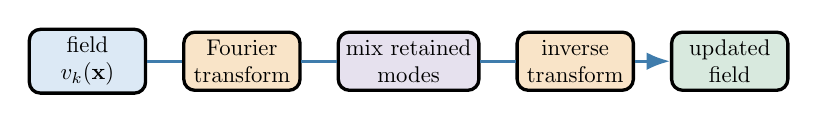
\begin{tikzpicture}[node distance=0.55cm,scale=0.82,transform shape]
    \node[box,fill=courselightblue] (v) {field\\\(v_k(\mathbf x)\)};
    \node[box,fill=courselightorange,right=of v] (fft) {Fourier\\transform};
    \node[box,fill=coursepurple!18,right=of fft] (mix) {mix retained\\modes};
    \node[box,fill=courselightorange,right=of mix] (ifft) {inverse\\transform};
    \node[box,fill=coursegreen!18,right=of ifft] (out) {updated\\field};
    \draw[flow] (v)--(fft)--(mix)--(ifft)--(out);
  \end{tikzpicture}
  \vspace{0.6cm}
  \begin{itemize}
    \item Fourier modes provide global receptive fields in one layer.
    \item Learned spectral weights act on feature channels mode by mode.
    \item A regular grid and periodic transform assumptions enter the implementation.
  \end{itemize}
\end{frame}

\begin{frame}{An FNO Layer Combines Spectral and Local Paths}
  \[
    \boxed{
    v_{k+1}(\mathbf x)
      =\sigma\!\left(
        W_kv_k(\mathbf x)
        +\mathcal F^{-1}\!\left(
          R_k(\boldsymbol\xi)\,\mathcal F[v_k](\boldsymbol\xi)
        \right)(\mathbf x)
      \right)}.
  \]
  \begin{itemize}
    \item \(W_k\): pointwise channel mixing.
    \item \(R_k(\boldsymbol\xi)\): learned matrix for retained mode \(\boldsymbol\xi\).
    \item \(\mathcal F^{-1}R_k\mathcal F\): nonlocal spectral convolution.
    \item Lifting and projection layers connect physical and hidden channels.
  \end{itemize}
\end{frame}

\begin{frame}{Mode Truncation Trades Detail for Efficiency}
  Retain only \(|\xi_j|\leq K_j\):
  \[
    R_k(\boldsymbol\xi)=0
    \quad\text{outside the retained band}.
  \]
  \centering
  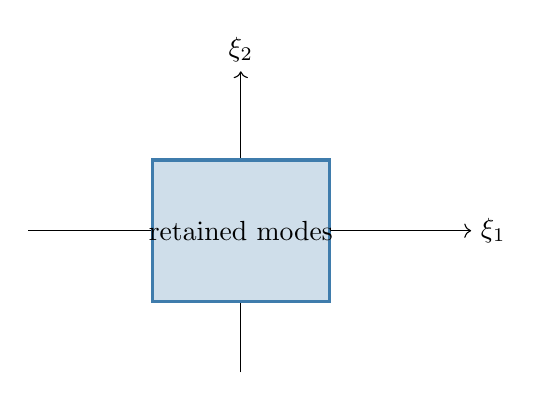
\begin{tikzpicture}[scale=0.45]
    \draw[->] (-6,0)--(6.5,0) node[right] {\(\xi_1\)};
    \draw[->] (0,-4)--(0,4.5) node[above] {\(\xi_2\)};
    \fill[courseblue!25] (-2.5,-2) rectangle (2.5,2);
    \draw[courseblue,very thick] (-2.5,-2) rectangle (2.5,2);
    \node at (0,0) {retained modes};
  \end{tikzpicture}
  \begin{itemize}
    \item Fewer modes reduce parameters and computation.
    \item Fine scales, discontinuities, and sharp boundaries need higher modes.
  \end{itemize}
\end{frame}

\begin{frame}{Operator Models Extrapolate Poorly Under Distribution Shift}
  Test changes may affect
  \begin{itemize}
    \item coefficient magnitude or correlation length,
    \item forcing frequency and amplitude,
    \item geometry and boundary conditions,
    \item temporal horizon,
    \item discretization and resolution.
  \end{itemize}
  \[
    a_{\mathrm{test}}\not\sim p_{\mathrm{train}}(a)
    \quad\Longrightarrow\quad
    \text{accuracy is not guaranteed}.
  \]
  \begin{itemize}
    \item Physics-inspired architecture does not remove statistical shift.
  \end{itemize}
\end{frame}

\begin{frame}{PINNs and Neural Operators Solve Different Problems}
  \begin{center}
  \begin{tabular}{lcc}
    \hline
      & PINN & Neural operator\\
    \hline
    Target & one solution \(u\) & map \(a\mapsto u\)\\
    Training & per instance & across instances\\
    Main supervision & residual/data & solution families\\
    New instance & retrain or adapt & forward evaluation\\
    Benefit & limited observations & repeated related solves\\
    \hline
  \end{tabular}
  \end{center}
  \begin{itemize}
    \item Neither dominates for every PDE workload.
  \end{itemize}
\end{frame}

\begin{frame}{Data and Physics Can Constrain Either Approach}
  \[
    L_{\mathrm{hybrid}}
      =L_{\mathrm{data}}
       +\lambda_rL_{\mathrm{residual}}
       +\lambda_cL_{\mathrm{conservation}}.
  \]
  \begin{itemize}
    \item A neural operator can be trained with solution data and PDE residuals.
    \item A PINN can use sparse observations in addition to equations.
    \item Hard architectural symmetries can complement soft physical penalties.
    \item Every added term creates a scale and optimization choice.
  \end{itemize}
\end{frame}

\begin{frame}{Established Numerical Solvers Are Essential Baselines}
  Compare
  \[
    \text{error},\quad
    \text{offline cost},\quad
    \text{per-query cost},\quad
    \text{memory},\quad
    \text{robustness}.
  \]
  \begin{itemize}
    \item PINNs should be compared with direct numerical solves for the same instance.
    \item Operators should include training-data generation in offline cost.
    \item Report speed only at matched accuracy and hardware.
    \item Verify convergence, conservation, and out-of-distribution behavior.
  \end{itemize}
\end{frame}

\begin{frame}{Physics Supplies Structure, Not Immunity}
  \begin{itemize}
    \item PINNs optimize a coordinate-based solution under differential constraints.
    \item Automatic differentiation evaluates derivatives of the represented field.
    \item Neural operators amortize a family of related PDE solves.
    \item DeepONet factorizes input-function and query-coordinate dependence.
    \item FNO learns global spectral mixing with truncated modes.
    \item Optimization, discretization, validation, and distribution shift remain central.
  \end{itemize}
\end{frame}

\end{document}
